\documentclass[a4paper,UKenglish,cleveref, autoref, thm-restate,anonymous]{lipics-v2021}

\hideLIPIcs  

\bibliographystyle{plainurl}

\ifx\authoranonymous\relax
\newcommand{\GITHUBURL}{(anonymised)}
\newcommand{\COFFEEURL}{(anonymised)}
\else
\newcommand{\GITHUBURL}{\url{https://github.com/songlarknet/pipit}}
\newcommand{\COFFEEURL}{\url{https://youtu.be/6IybbQFPOl8}}
\fi

\usepackage{mathtools}
\usepackage{mathpartir}

\usepackage{stmaryrd}

\usepackage{wasysym}
\usepackage{underscore}

\usepackage{style/utils}
\usepackage{style/code}
\usepackage{style/proof}
\usepackage{style/keywords}
\usepackage{style/judgements}


\title{Pipit on the Post: Proving Pre- and Post-conditions of Reactive Systems}


\author{Amos Robinson}{Australian National University, Canberra, Australia}{amos.robinson@anu.edu.au}{https://orcid.org/0009-0004-4837-4981}{}

\author{Alex Potanin}{Australian National University, Canberra, Australia}{alex.potanin@anu.edu.au}{https://orcid.org/0000-0002-4242-2725}{}

\authorrunning{A. Robinson and A. Potanin}
\Copyright{Amos Robinson and Alex Potanin}
\ccsdesc[500]{Computer systems organization~Real-time languages}
\ccsdesc[500]{Theory of computation~Program verification}
\ccsdesc[500]{Software and its engineering~Specialized application languages}
\keywords{Lustre, streaming, reactive, verification}



\begin{document}

\maketitle

\begin{abstract}
  Reactive languages such as Lustre and Scade are used to implement safety-critical control systems; proving such programs correct and having the proved properties apply to the compiled code is therefore equally critical.
  We introduce Pipit, a small reactive language embedded in \fstar{}, designed for verifying control systems and executing them in real-time.
  Pipit includes a verified translation to transition systems; by reusing \fstar{}'s existing proof automation, certain safety properties can be automatically proved by k-induction on the transition system.
  Pipit can also generate executable code in a subset of \fstar{} which is suitable for compilation and real-time execution on embedded devices.
  The executable code is deterministic and total and preserves the semantics of the original program.
\end{abstract}


% \makeatactive


\section{Introduction}
Safety-critical control systems, such as the anti-lock braking systems that are present in most cars today, need to be correct and execute in real-time.
One approach, favoured by parts of the aerospace industry, is to implement the controllers in a high-level language such as Lustre~\cite{caspi1995functional} or Scade~\cite{colaco2017scade}, and verify that the implementations satisfy the high-level specification using a model-checker, such as Kind2~\cite{champion2016kind2}.
These model-checkers can prove many interesting safety properties automatically, but do not provide many options for manual proofs when the automated proof techniques fail.
Additionally, the semantics used by the model-checker may not match the semantics of the compiled code, in which case properties proved do not necessarily hold on the real system.
This mismatch may occur even when the compiler has been verified to be correct, as in the case of Vélus~\cite{bourke2017formally}.
For example, in Vélus, integer division rounds towards zero, matching the semantics of C; however, integer division in Kind2 rounds to negative infinity, matching SMT-lib~\cite{BarFT2016SMTLIB,kind2023intdiv}.

To be confident that our proofs hold on the real system, we need a single shared semantics for the compiler and the prover.
In this paper we introduce Pipit\footnote{Implementation available at \GITHUBURL}, an embedded domain-specific language for implementing and verifying controllers in \fstar{}.
Pipit aims to provide a high-level language based on Lustre, while reusing \fstar{}'s proof automation and manual proofs for verifying controllers~\cite{martinez2019meta}, and using \lowstar{}'s C-code generation for real-time execution~\cite{protzenko2017verified}.
To verify programs, Pipit translates its expression language to a transition system for k-inductive proofs, which is verified to be an abstraction of the original semantics.
To execute programs, Pipit can generate executable code, which is total and semantics-preserving.



In this paper, we make the following contributions:

\begin{itemize}
  \item we motivate the need to combine manual and automated proofs of reactive systems with a strong specification language (\autoref{s:motivation});
  \item we introduce Pipit, a minimal reactive language that supports rely-guarantee contracts and properties; crucially, proof obligations are annotated with a status --- \emph{valid} or \emph{deferred} --- allowing proofs to be delayed until more is known of the program context (\autoref{s:core});
  \item we describe a \emph{checked semantics} for Pipit; after checking deferred properties, programs are \emph{blessed}, which marks their properties as valid (\autoref{s:core:checked});
  \item we describe an encoding of transition systems that can express under-specified rely-guarantee contracts as functions rather than relations; composing functions results in simpler transition systems (\autoref{s:transition});
  \item we identify the invariants and lemmas required to prove that the abstract transition system is an abstraction of the original semantics (\autoref{s:core:causality}, \autoref{s:transition:proof});
  \item similarly, we offer a mechanised proof that the executable transition system preserves the original semantics (\autoref{s:extraction});
  \item finally, we evaluate Pipit by implementing the high-level logic of a Time-Triggered Controller Area Network (TTCAN) bus driver and verifying an abstract model of a key component (\autoref{s:evaluation}).
\end{itemize}
 

\section{Pipit for time-triggered networks}
\label{s:motivation}

To introduce Pipit, we consider a \emph{time-triggered} network driver, which has a static schedule dictating the network traffic, and which all nodes on the network must adhere to.
This driver is a simplification of the Time-Triggered Controller Area Network (TTCAN) bus specification \cite{fuehrer2001time} which we will discuss further in \autoref{s:evaluation}.

At a high level, the network schedule is described by a \emph{system matrix} which consists of rows of \emph{basic cycles}.
Each basic cycle consists of a sequence of actions to be performed at specific time-marks.
Actions in the schedule may not be relevant to all nodes; the node's \emph{node matrix} contains only the relevant actions.
The node matrix is represented in memory by a \emph{triggers array} containing triggers sorted by their time-marks; trigger actions include sending and receiving application-specific messages, sending reference messages, and triggering `watch' alerts.
Reference messages start a new basic cycle; a subset of nodes, designated as leaders, send reference messages to synchronise the network.
Watch alerts are generally placed after an expected reference message to signal an error if no reference message is received.

\autoref{f:tt-systemmatrix-ok} (left) shows an example node matrix for a non-leader node.
The matrix consists of two basic cycles C0 and C1 with messages sent at time-marks 0, 1 and 2.
The node expects to receive a reference message at time-mark 7; the watch at time-mark 9 allows a grace period before triggering an error if the reference message is not received.
\autoref{f:tt-systemmatrix-ok} (right) shows the corresponding triggers array.

\begin{figure}
  \begin{minipage}{0.5\textwidth}
\resizebox{\textwidth}{!}{
\begin{tabular}{r|ccccc}
   & TM0 & TM1 & TM2 & $\cdots$ & TM9 \\
  \hline
  C0 & SEND A & SEND B & - & $\cdots$ & WATCH \\
  C1 & SEND A & - & SEND C & $\cdots$ & WATCH
\end{tabular}}
\end{minipage}
\begin{minipage}{0.49\textwidth}
\scriptsize
\begin{verbatim}
 0:{ time = 0; enabled = {C0,C1}; action = SEND(A); }
 1:{ time = 1; enabled = {C0};    action = SEND(B); }
 2:{ time = 2; enabled = {C1};    action = SEND(C); }
 3:{ time = 9; enabled = {C0,C1}; action = WATCH;   }
\end{verbatim}
\end{minipage}

\caption{Left: node matrix; right: corresponding triggers array configuration}
\label{f:tt-systemmatrix-ok}
\end{figure}

The network has strict timing requirements which prohibit the driver from looping through the entire triggers array at each time-mark.
Instead, the driver maintains an index that refers to the current trigger.
At each time-mark, the driver checks if the current trigger has expired or is inactive, and if so, it increments the index.

\subsection{Deferring and proving properties}

We implement a streaming function \emph{count_when} to maintain the index into the triggers array; the function takes a constant natural number \emph{max} and a stream of booleans \emph{inc}.
At each step, \emph{count_when} checks whether the current increment flag is true; if so, it increments the previous counter, saturating at the maximum; otherwise, it leaves the counter as-is.

\begin{tabbing}
  \tt{MM}\= \tt{MM} \= \kill
  \tt{let} count_when ($\textit{max}$: $\NN$) ($\textit{inc}$: stream $\BB$): stream $\NN$ = \\
    \> $\tt{rec}~\rawbind{\textit{count}}{}$ \\
    \> \> $\xcheckP{\PSUnknown}{(0 \le \textit{count} \le \textit{max})}$; \\
    \> \> \tt{let} $\textit{count'}$ \tt{=} $(0~\tt{fby}~\textit{count}) + (\tt{if}~\textit{inc}~\tt{then}~1~\tt{else}~0)$ \tt{in} \\
    \> \> \tt{if } $\textit{count'} \ge \textit{max}$ \tt{then} $\textit{max}$  \tt{else} $\textit{count'}$
\end{tabbing}

The implementation of \emph{count_when} first defines a recursive stream, \emph{count}, which states an invariant about the count before defining the incremented stream \emph{count'}.
Inside \emph{count'}, the syntax $0~\tt{fby}~\textit{count}$ is read as ``the initial value of zero \emph{followed by} the previous count''.

The syntax $\xcheckP{\PSUnknown}{(0 \le \textit{count} \le \textit{max})}$ asserts that the count is within the range $[0, \textit{max}]$.
The subscript $\PSUnknown$ on the check is the \emph{property status}, which in this case denotes that the assertion has been stated, but it is not yet known whether it holds.
A property status of $\PSValid$, on the other hand, denotes that a property has been proved to hold.
These property statuses are used to defer checking properties until enough is known about the environment, and to avoid rechecking properties that have already been proven.
In practice, the user does not explicitly specify property statuses in the source language.
The stated property $(0 \le \textit{count} \le \textit{max})$ is a stream of booleans which must always be true.
Non-streaming operations such as $\le$ are implicitly lifted to streaming operations, and non-streaming values such as $0$ and $\textit{max}$ are implicitly lifted to constant streams.

We defer the proof of the property here because, at the point of stating the property inside the \tt{rec} combinator, we don't yet have a concrete definition for the count variable.
In this case, we could have instead deferred the \emph{statement} of the property by introducing a let-binding for the recursive count and putting the \tt{check} outside of the \tt{rec} combinator.
However, it is not always possible to defer property statements: for example, when calling other streaming functions that have their own preconditions, it may not be possible to move the function call outside of its enclosing \tt{rec}.


Pipit is an embedded domain-specific language.
The program above is really syntactic sugar for an \fstar{} program that takes a natural number and constructs a Pipit core expression with a free boolean variable.
We will discuss the details of the core language in \autoref{s:core}, but for now we focus on the source program with some minor embedding details omitted.

To actually prove the property above, we use the meta-language \fstar{}'s tactics to translate the program into a transition system and prove the property inductively on the system.
Finally, we \emph{bless} the expression, which marks the properties as valid ($[\PSUnknown := \PSValid]$).
Blessing is an intensional operation that traverses the expression and updates the internal metadata, but does not affect the runtime semantics.

\begin{tabbing}
  \tt{MM}\= \tt{MM} \= \kill
  \tt{let} $\mbox{count_when}_{\PSValid}$ ($\textit{max}$: $\NN$): stream $\BB$ $\to$ stream $\NN$ = \\
    \> \tt{let} $\textit{system} = \mbox{System.translate}_1 (\mbox{count_when}~\textit{max})$ \tt{in} \\
    \> \tt{assert} (System.inductive_check $\textit{system}$) \tt{by} (pipit_simplify ()); \\
    \> $\tt{bless}_1$ $(\mbox{count_when}~\textit{max})$
\end{tabbing}

The subscript 1 in the translation to transition system and blessing operations refers to the fact that the stream function has one stream parameter.
The \emph{pipit_simplify} tactic in the assertion performs normalisation-by-evaluation to simplify away the translation to a first-order transition system; \fstar{}'s proof-by-SMT can then solve the inductive check directly.


Callers of \emph{count_when} can now use the validated variant without needing to re-prove the count-range property.
In a dedicated model-checker such as Kind2 \cite{champion2016kind2} or Lesar \cite{raymond2008synchronous}, this kind of bookkeeping would all be performed under-the-hood.
By embedding Pipit in a general-purpose theorem prover, we move some of the bookkeeping burden onto the user; however, we have increased confidence that the compiled code matches the verified code and, as we shall see, we also have access to a rich specification language.


\subsection{Restrictions on the triggers array}

Our driver may fall behind when trying to execute certain schedules, as the driver only processes one trigger per time-mark.
To ensure that the schedule can be executed on time, the triggers array must allow sufficient time for the driver to skip over any disabled triggers before the next enabled trigger starts.

Recall our concrete triggers array from \autoref{f:tt-systemmatrix-ok}, which contained trigger 1 (SEND B at time-mark 1 on cycle C0), and trigger 2 (SEND C at time-mark 2 on cycle C1).
We could postpone trigger 1 to send B at time-mark 2, as the corresponding cell in the node matrix is empty.
However, we \emph{cannot} bring the trigger at index 2 forward to send message C at time-mark 1, as it takes two steps to reach trigger 2 from the start of the array.

We impose three restrictions on \emph{valid} triggers arrays: the time-marks must be sorted; there must be an adequate time-gap between any two triggers that are enabled on the same cycle index; and each trigger's time-mark must be greater-than-or-equal to its index, so that it is reachable in time from the start of the array.

With these restrictions in place, we prove a lemma \emph{lemma_can_reach_next}, which states that for all valid cycle indices and trigger indices, if the current trigger is enabled in the current cycle and there is another enabled trigger scheduled to occur somewhere in the array after the current one, then there is an adequate time-gap to allow the driver to skip over any disabled triggers in-between.
These properties are straightforward in a theorem prover, but are difficult to state in a model-checker with a limited specification language.

\subsection{Instantiating lemmas and defining contracts}
\label{s:motivation:contract}

We can now implement the trigger-fetch logic, which keeps track of the current trigger.
We use the \emph{count_when} streaming function to define the index of the current trigger; we tell \emph{count_when} to increment the index whenever the previous index has expired or is inactive in the current basic cycle.
We simplify our presentation here and only consider a constant cycle: the real system presented in \autoref{s:evaluation} has some extra complexity such as resetting the index, incrementing the cycle index at the start of a new cycle, and using machine integers.

\begin{tabbing}
  \tt{MM}\= \tt{MM} \= \tt{let index} \= \kill
  \tt{let} trigger_fetch ($\textit{cycle}$: $\NN$) ($\textit{time}$: stream $\NN$): stream $\NN$ = \\
    \> $\tt{rec } \textit{index}.$ \\
    \> \> $\tt{let } \textit{inc} = \text{false} \tt{ fby } ((\text{time_mark}~\textit{index}) \le \textit{time} ~\vee~ \neg (\text{enabled}~\textit{index}~\textit{cycle})) \tt{ in}$\\
    \> \> $\tt{let } \textit{index} = \mbox{count_when}_{\PSValid}~\text{trigger_count}~\textit{inc} \tt{ in}$ \\
    \> \> $\text{pose}~(\text{lemma_can_reach_next}~\textit{cycle}~\textit{index})$; \\
    \> \> $\xcheckP{\PSUnknown}{(\text{can_reach_next_active}~\textit{cycle}~\textit{time}~\textit{index})}$; \\
    \> \> $\textit{index}$
\end{tabbing}

The \emph{trigger_fetch} function takes a static cycle index and a stream denoting the current time.
The increment flag and the index are mutually dependent --- the increment flag depends on the previous value of the index, while the index depends on the current value of the increment flag --- so we introduce a recursive stream for the index.
We allow the index to go one past the end of the array to denote that there are no more triggers.

We use the $\textit{pose}$ helper function to lift the \emph{lemma_can_reach_next} lemma to a streaming context and instantiate it.
We then state an invariant as a deferred property.
Informally, the invariant states that, either the current active trigger is not late, or the next active trigger after the current index is in the future and we can reach it in time.

With the explicitly instantiated lemma, we can prove the streaming invariant by straightforward induction on the transition system.
To help compose this function with the rest of the system, we also abstract over the details of the trigger-fetch mechanism by introducing a rely-guarantee contract for \emph{trigger_fetch}.
The contract we state is that if we are called once per time-mark then we guarantee that we never encounter a late trigger.


\begin{tabbing}
  \tt{MM}\= \tt{MM} \= \tt{MMMMMMMMMMMMM} \= \kill
  \tt{let} $\text{trigger_fetch}_{\PSValid}$ ($\textit{cycle}$: $\NN$): $\stream \NN \to \stream \NN$ = \\
  \> \tt{let} $\textit{contract} = \text{Contract.contract_of_stream}_1$ \{ \\
  \> \> \tt{rely} = $(\lambda \textit{time}.~ \textit{time} = \xfby{0}{(\textit{time} + 1)});$ \\
  \> \> \tt{guar} = $(\lambda \textit{time index}.~ (\text{index_valid}~\textit{index} \wedge \text{enabled}~\textit{index}~\textit{cycle})$ \\
  \> \> \> $\implies (\text{time_mark}~\textit{index}) \ge \textit{time});$ \\
  \> \> \tt{body} = $(\lambda \textit{time}.~ \text{trigger_fetch}~\textit{cycle}~\textit{time} );$ \\
  \> \} \tt{in} \\
  \> \tt{assert} $(\text{Contract.inductive_check}~\textit{contract})$ \tt{by} (pipit_simplify ()); \\
  \> $\text{Contract.stream_of_contract}_1~\textit{contract}$
\end{tabbing}

In the implementation of the validated variant of \emph{trigger_fetch}, we first construct the contract from streaming functions.
The $\text{Contract.contract_of_stream}_1$ combinator describes a contract with one input (the time stream), and takes stream transformers for each of the rely, guarantee and body.
The combinator transforms the surface syntax into core expressions.
The assertion $(\text{Contract.inductive_check}~\textit{contract})$ then translates the expressions into a transition system, and checks that if the rely always holds then the guarantee always holds, and that the as-yet-unchecked subproperties hold.
Finally, $\text{Contract.stream_of_contract}_1$ blesses the core expression and converts it back to a stream transformer, so it can be easily used by other parts of the program.

The key distinction between our streaming rely-guarantee contracts and imperative pre-post contracts is that the rely and guarantee are both \emph{streams} of booleans, rather than instantaneous predicates.
In this case, the rely $(\textit{time} = \xfby{0}{(\textit{time} + 1)})$ checks that the current time is exactly one time-mark after the time at the previous \emph{tick} of computation.
Expressing such a rely in an imperative setting would require extra encoding, as preconditions in imperative languages do not generally have an innate notion of the previous value with respect to a global shared clock.

When \emph{trigger_fetch} is used in other parts of the program, the caller must ensure that the environment satisfies the rely clause.
In the core language, this is tracked by another deferred property status attached to the contract; we will discuss this further in \autoref{s:core}.
 

\section{Pipit core language}
\label{s:core}

\begin{figure}
  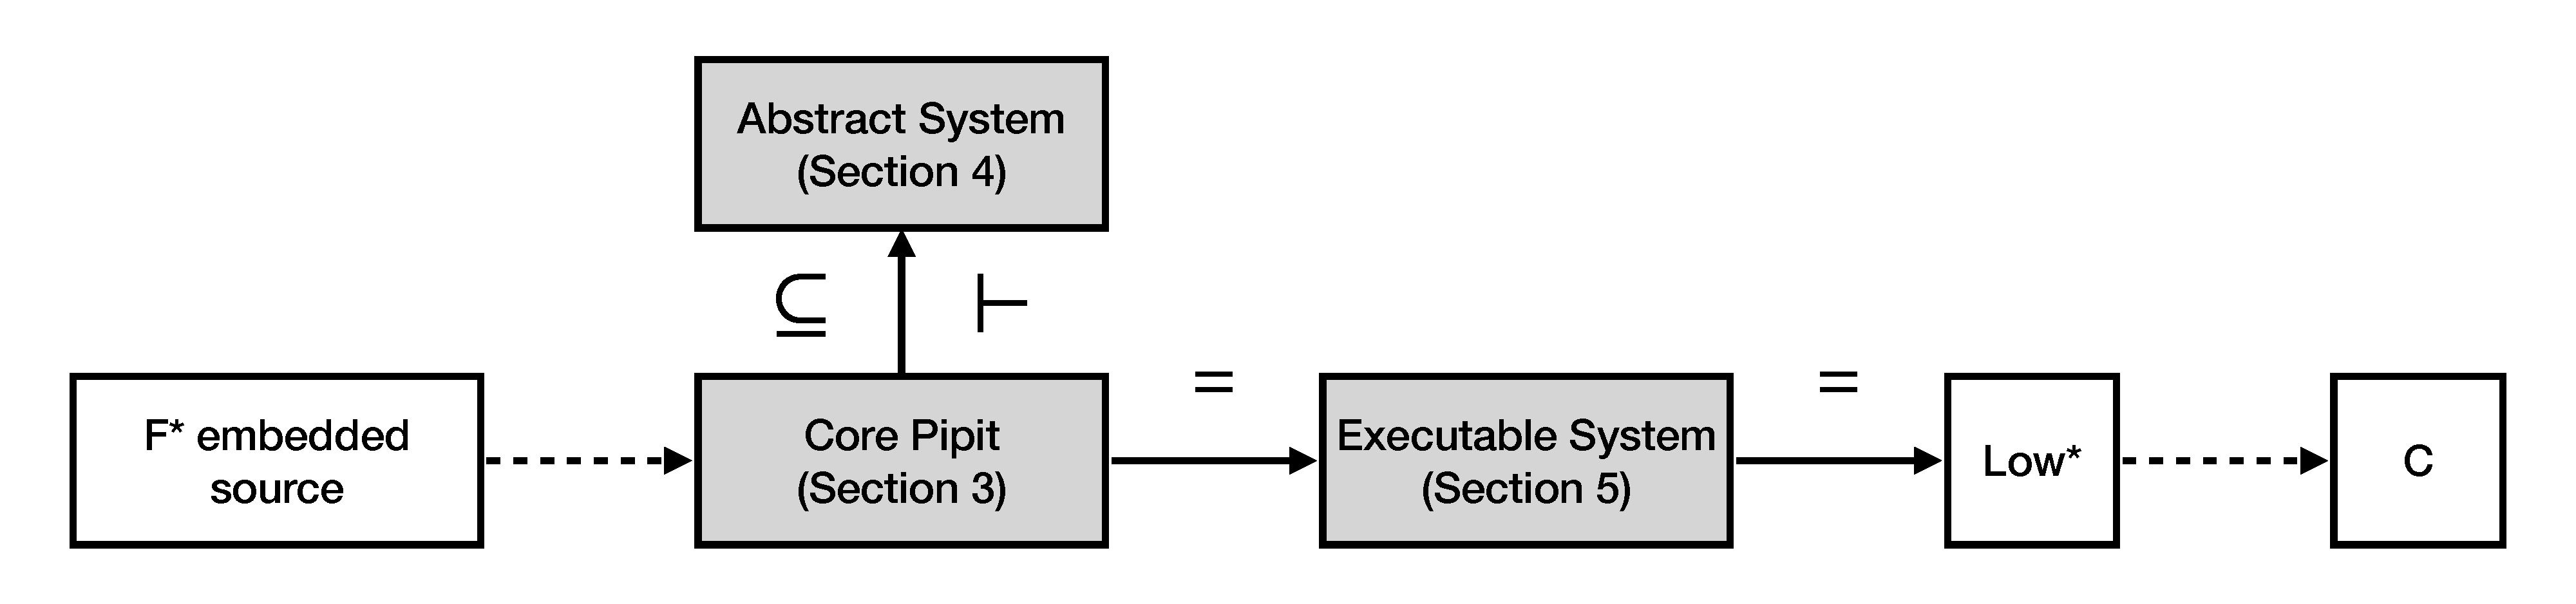
\includegraphics[width=\textwidth]{figures/core-structure-1920x450.pdf}
\caption{Architecture of Pipit. The gray boxes and solid arrows are defined in this paper. The white boxes and dashed arrows are trusted components. The labels denote verified properties of the translation: abstraction~($\subseteq$), entailment of proof obligations~($\vdash$), and equivalence~($=$).
}
\label{f:core:structure}
\end{figure}
 
We now introduce the core Pipit language.
Note that this form differs slightly from the surface syntax presented earlier in \autoref{s:motivation}, which used the syntax of the metalanguage \fstar{}, as well as including proofs in \fstar{} itself.


\autoref{f:core:structure} shows the high-level architecture of Pipit.
On the left-hand-side, the surface syntax embedded in \fstar{} is shown; this includes some Pipit-specific syntactic sugar.
The translation from the surface syntax to the core language is trusted.
There are two targets from the core language: abstract transition systems for verification, and executable transition systems for extraction to C.
The translation to abstract systems is verified to be an abstraction according to the dynamic semantics (\autoref{s:core:dynamic}).
The translation to abstract systems also generates proof obligations, which are verified to correspond to the proof obligations on the original program.
The translation to executable transition systems is proven to be semantics-preserving, as is the subsequent translation to \lowstar{}.
The translation from \lowstar{} to C is external to this paper and forms part of our trusted computing base.


\autoref{f:core-grammar} defines the grammar of Pipit.
The expression form $e$ includes standard syntax for values ($v$), variables ($x$) and primitive applications ($p(\ov{e})$).
Most of the expression forms were introduced informally in \autoref{s:motivation} and correspond to the clock-free expressions of Lustre~\cite{caspi1995functional}.



\begin{figure}
  \[
  \begin{array}{lrlr}
    e, e' & := & v ~|~ x ~|~ p(\ov{e}) & \mbox{(values, variables and operations)} \\
          & | & \xfby{v}{e} ~|~ \xrec{x}{e[x]} & \mbox{(delayed and recursive streams)} \\ & | & \xlet{x}{e}{e'[x]} & \mbox{(let-expressions)}\\
          & | & \xcheckP{\PStatus}{e_{\text{prop}}} & \mbox{(checked properties)} \\
          & | & \xcontractP{\PStatus}{\erely}{\ebody}{\rawbind{x}{\eguar[x]}} & \mbox{(rely-guarantee contracts)} \\
\\
    v & := & n \in \mathbb{N} ~|~ b \in \mathbb{B} ~|~ r \in \mathbb{R} ~|~ \hdots  & \mbox{(values)} \\
    p & := & (+) ~|~ (-) ~|~ (\times) ~|~ \tt{if-then-else} ~|~ \hdots & \mbox{(primitives)} \\
    \\
    \PStatus & := & \PSValid ~|~ \PSUnknown & \mbox{(property statuses: valid or unknown)}\\
    \\
    V & := & \cdot ~|~ V;v & \mbox{(streams of values)} \\
    \sigma & := & \sgl{\ov{x \mapsto v}} & \mbox{(heaps)} \\
    \Sigma & := & \cdot ~|~ \Sigma;\sigma & \mbox{(streaming history environments)} \\
\tau, \tau' & := & \mathbb{N} ~|~ \mathbb{B} ~|~ \tau \times \tau ~|~ \hdots & \mbox{(value types)} \\
    \Gamma & := & \cdot ~|~ x : \tau, \Gamma & \mbox{(type environments)}  \\
    \end{array}
  \]
  \caption{Core grammar: expressions $e$, values $v$, primitive operations $p$, and property statuses $\PStatus$.}
  \label{f:core-grammar}
\end{figure} 
The expression syntax for delayed streams ($\xfby{v}{e}$) denotes the previous value of the stream $e$, with an initial value of $v$ when there is no previous value.


Recursive streams are defined using the fixpoint operator ($\xrec{x}{e[x]}$); the syntax $e[x]$ means that the variable $x$ can occur in $e$.
As in Lustre, recursive streams can only refer to their previous values and must be \emph{guarded} by a delay: the stream $(\xrec{x}{\xfby{0}{(x + 1)}})$ is well-defined and counts from zero up, but the stream $(\xrec{x}{x + 1})$ is invalid and has no computational interpretation.
This form of recursion differs slightly from standard Lustre, which uses a set of mutually-recursive bindings.
Although we cannot express mutually-recursive bindings in the core syntax here, we can express them as a notation on the surface syntax by combining the bindings together into a record or tuple.

Checked properties and contracts are annotated with their property status $\PStatus$, which can either be valid ($\PSValid$) or unknown ($\PSUnknown$).
For checked properies $\xcheckP{\PStatus}{e}$, the property status denotes whether the property has been proved to be valid.

Contracts $\xcontractP{\PStatus}{\erely}{\ebody}{\rawbind{x}\eguar[x]}$ allow modular reasoning by replacing the implementation with an abstract specification.
Contracts involve two verification conditions.
Firstly, when a contract is \emph{defined}, the definer must prove that the body satisfies the contract: roughly, if $\erely$ is always true, then $\eguar[x := \ebody]$ is always true.
Secondly, when a contract is \emph{instantiated}, the caller must prove that the environment satisfies the precondition: that is, $\erely$ is always true.
Conceptually, then, a contract could have two property statuses: one for the definition and one for the instantiation.
However, in practice, it is not useful to defer the proof of a contract definition --- one could achieve a similar effect by replacing the contract with its implementation.
For this reason, we only annotate contracts with one property status, which denotes whether the instantiation has been proved to satisfy the precondition.

For example, the core expression $\sumrec$ computes the sum of values from a stream of integers \emph{ints} by defining a recursive stream $\sumvar$, which is delayed and given an initial value of zero.
If we were to use this sum in a context that required a strictly positive integer, we could give it a contract that states that if the input stream is always positive, then the resulting sum is also positive:
$$
\sumcontract
$$
To be considered a valid program, we must prove that the contract definition itself holds, as with our earlier contract (\autoref{s:motivation:contract}).
The unknown property status here allows us to defer the caller's proof that the input stream is always positive until the contract is used.



The remaining grammatical constructs of \autoref{f:core-grammar} describe streams, value environments, types and type environments.
Streams $V$ are represented as a sequence of values; streaming history environments $\Sigma$ are streams of heaps.
Types $\tau$ and type environments $\Gamma$ are standard.
For the presentation of the formal grammar here, we consider only a fixed set of values and primitives; in practice, the implementation is parameterised by a primitive table which we extend with immutable array operations for the TTCAN driver logic in \autoref{s:evaluation}.



\begin{figure}
  \begin{mathpar}
    \boxed{\typing{\Gamma}{e}{\tau}}
\end{mathpar}

  \begin{mathpar}
    \ruleIN{
      \mtypingval{v}{\tau}
    }{
      \typing{\Gamma}{v}{\tau}
    }{TValue}

    \ruleAx{\typing{\Gamma, x: \tau, \Gamma'}{x}{\tau}}{TVar}

    \ruleIN{
      \mtypingprim{p}{(\tau_1 \times \dots \times \tau_n) \to \tau'}
      \qquad
      \typing{\Gamma}{e_1}{\tau_1}
      \quad \hdots \quad
      \typing{\Gamma}{e_n}{\tau_n}
    }{\typing{\Gamma}{p(\ov{e})}{\tau'}}{TPrim}

    \ruleIN{
      \mtypingval{v}{\tau}
      \qquad
      \typing{\Gamma}{e'}{\tau}
    }{
      \typing{\Gamma}{\xfby{v}{e'}}{\tau}
    }{TFby}

\ruleIN{
      \typing{\Gamma, x : \tau}{e}{\tau}
    }{
      \typing{\Gamma}{\xrec{x}{e[x]}}{\tau}
    }{TRec}

    \ruleIN{
      \typing{\Gamma}{e}{\tau}
      \qquad
      \typing{\Gamma, x : \tau}{e'}{\tau'}
    }{
      \typing{\Gamma}{\xlet{x}{e}{e'[x]}}{\tau'}
    }{TLet}

    \ruleIN{
      \typing{\Gamma}{e}{\mathbb{B}}
    }{
      \typing{\Gamma}{\xcheckP{\PStatus}{e}}{\tt{unit}}
    }{TCheck}
  \and
    \ruleIN{
      \typing{\Gamma}{\erely}{\mathbb{B}}
      \qquad
      \typing{\Gamma}{\ebody}{\tau}
      \qquad
      \typing{\Gamma, x: \tau}{\eguar}{\mathbb{B}}
    }{
      \typing{\Gamma}{\xcontractP{\PStatus}{\erely}{\ebody}{\rawbind{x}{\eguar[x]}}}{\tau}
    }{TContract}
  \end{mathpar}

  \caption{Typing rules for Pipit; the judgment $\typing{\Gamma}{e}{\tau}$ denotes that expression $e$ describes a \emph{stream} of values of type $\tau$. Auxiliary functions are used for values and primitive operations.}\label{f:core-typing}
\end{figure} 
We define the typing judgments for Pipit in \autoref{f:core-typing}.
Most of the typing rules are standard for an unclocked Lustre.
The typing judgment $\typing{\Gamma}{e}{\tau}$ denotes that, in an environment of streams $\Gamma$, expression $e$ denotes a stream of type $\tau$.
This core typing judgment differs from the surface syntax used in \autoref{s:motivation}, which used an explicit stream type; for the core language, we instead assume that everything is a stream.

We use an auxiliary function $\mtypingval{v}{\tau}$ to denote that value $v$ has type $\tau$; for primitives $\mtypingprim{p}{(\tau_1 \times \cdots \hdots \times \tau_n) \to \tau'}$ denotes that $p$ takes arguments of type $\tau_i$ and returns a result of type $\tau'$.
Primitives are pure, non-streaming functions.

Rules \textsc{TValue}, \textsc{TVar}, \textsc{TPrim} and \textsc{TLet} are standard.

Rule \textsc{TFby} states that expression $\xfby{v}{e}$ requires both $v$ and $e$ to have equal types.

Rule \textsc{TRec} states that a recursive stream $\xrec{x}{e}$ has the recursive stream bound inside $e$.
The recursion must also be guarded, in that any recursive references to $x$ are delayed, but this requirement is performed as a separate syntactic check described in \autoref{s:core:causality}.

Rule \textsc{TCheck} states that checked properties $\xcheckP{\PStatus}{e}$ require a boolean property $e$.

Finally, rule \textsc{TContract} applies for a contract $\xcontractP{\PStatus}{\erely}{\ebody}{\rawbind{x}\eguar[x]}$ with a body expression of type $\tau$.
The overall expression has result type $\tau$.
Both rely and guarantee must be boolean expressions, and the guarantee can refer to the result as $x$.

\subsection{Dynamic semantics}
\label{s:core:dynamic}


\begin{figure}[t]
  \begin{mathpar}
    \boxed{\bigstep{\Sigma}{e}{v}}
  \end{mathpar}
  \begin{mathpar}
    \ruleAx{\bigstep{\Sigma; \sigma}{x}{\sigma(x)}}{Var}
    \quad
    \ruleAx{\bigstep{\Sigma}{v}{v}}{Value}

    \ruleIN{
      \bigstep{\Sigma}{e'[x := e]}{v}
    }{
      \bigstep{\Sigma}{\xlet{x}{e}{e'[x]}}{v}
    }{Let}

    \ruleIN{
      \bigstep{\Sigma}{e_1}{v_1} \quad \hdots \quad
      \bigstep{\Sigma}{e_n}{v_n}
    }{\bigstep{\Sigma}{p(\ov{e})}{\text{prim-sem}(p, \ov{v})}}{Prim}




  \ruleAx{\bigstep{\sigma}{\xfby{v}{e'}}{v}}{$\mbox{Fby}_1$}
    \quad
    \ruleIN{\text{length}(\Sigma) > 0 \and \bigstep{\Sigma}{e'}{v'}}{\bigstep{\Sigma; \sigma}{\xfby{v}{e'}}{v'}}{$\mbox{Fby}_S$}



    \ruleIN{
      \bigstep{\Sigma}{e[x := \xrec{x}{e}]}{v}
    }{
      \bigstep{\Sigma}{\xrec{x}{e[x]}}{v}
    }{Rec}

    \ruleIN{
}{
      \bigstep{\Sigma}{\xcheckP{\PStatus}{e}}{()}
    }{Check}

    \ruleIN{
      \bigstep{\Sigma}{\ebody}{v}
    }{
      \bigstep{\Sigma}{\xcontractP{\PStatus}{\erely}{\ebody}{\rawbind{x}{\eguar[x]}}}{v}
    }{Contract}
  \end{mathpar}

  \begin{mathpar}
    \boxed{\bigsteps{\Sigma}{e}{V}}

    \boxed{\bigstepalways{\Sigma}{e}}
  \end{mathpar}
  \begin{mathpar}
    \ruleAx{\bigsteps{\cdot}{e}{\cdot}}{$\mbox{Steps}_0$}


    \ruleIN{
      \bigstep{\Sigma}{e}{V}
      \and
      \bigstep{\Sigma; \sigma}{e}{v}
    }{\bigstep{\Sigma; \sigma}{e}{V; v}}{$\mbox{Steps}_S$}

    \ruleIN{\bigsteps{\Sigma}{e}{\true; \hdots}}{\bigstepalways{\Sigma}{e}}{Always}
  \end{mathpar}


  \caption{Dynamic semantics for Pipit; the judgment form $\bigstep{\Sigma}{e}{v}$ denotes that evaluating expression $e$ under streaming history $\Sigma$ results in value $v$.}\label{f:core-bigstep}
\end{figure}
 
The dynamic semantics of Pipit are defined in \autoref{f:core-bigstep}.
We present our semantics in a big-step form.
This differs somewhat from traditional \emph{reactive} semantics of Lustre~\cite{caspi1995functional}.
Our big-step semantics emphasises the equational nature of Pipit, as it is substitution-based and syntax-directed, while the reactive semantics emphasises the finite-state streaming execution of the system.
We use transition systems for reasoning about the finite-state execution (\autoref{s:transition}), which is fairly standard~\cite{brun2023equation,champion2016kind2,raymond2008synchronous}.
Previous work on the {\sc W-calculus}~\cite{gallego2021w} for linear digital-signal-processing filters makes a similar distinction and provides a non-streaming semantics for reasoning about programs and a streaming semantics for executing programs.


The judgment form $\bigstep{\Sigma}{e}{v}$ denotes that expression $e$ evaluates to value $v$ under streaming history $\Sigma$.
The streaming history is a stream of heaps; in practice, we only evaluate expressions with a non-empty streaming history.

At a high level, evaluation unfolds recursive streams to determine a value.
For example, to evaluate the earlier sum example with input $\textit{ints} = [1; 2]$, we start with the judgment:
$$
\bigstep{\sumintsonetwo}{\sumrec}{v}
$$

First, we unfold the recursive stream one step to get $(\xfby{0}{\sumrec}) + \textit{ints}$.
Evaluation of primitives is standard.
To evaluate variables, we look for the variable in the current (rightmost) heap:
$$
\ruleIN{
}{
  \bigstep{\sumintsonetwo}{\textit{ints}}{2}
}{Var}
$$

For delays, we discard the current heap and continue evaluation with the history prefix:
$$
\ruleIN{
  \bigstep{\sgl{\textit{ints} \mapsto 1}}{\sumrec}{1}
}{
  \bigstep{\sumintsonetwo}{\xfby{0}{\sumrec}}{1}
}{$\mbox{Fby}_S$}
$$

Returning to \autoref{f:core-bigstep},
rule {\sc Var} evalutes a variable $x$ under some non-empty stream history $\Sigma; \sigma$, where $\sigma$ is the most recent heap.
Rules {\sc Value} and {\sc Let} are standard.
Rule {\sc Prim} evaluates a primitive $p$ applied to many arguments $e_1$ to $e_n$ by evaluating each argument separately; we then apply the primitive with prim-sem metafunction.


For delay expressions $\xfby{v}{e}$, we have two cases depending on whether there is a previous value.
When there is no previous value -- the streaming history only contains the current heap -- rule $\textsc{Fby}_1$ evaluates to the default value $v$.
Otherwise, rule $\textsc{Fby}_S$ applies; we evaluate the previous value of $e$ by discarding the most recent entry from the streaming history.

Rule {\sc Rec} evaluates a recursive stream $\xrec{x}{e}$ by unfolding the recursion one step.
For causal expressions (\autoref{s:core:causality}), where each recursive occurrence of $x$ is guarded by a followed-by, this unfolding eventually terminates as each followed-by shortens the history.

Rule {\sc Check} ignores the property when evaluating check expressions.
We do not dynamically check the property here; this is done in the checked semantics (\autoref{s:core:checked}).

Similarly, rule {\sc Contract} ignores preconditions and postconditions when evaluating contracts.
From an abstraction perspective, it would be valid to return an arbitrary value that satisfies the contract.
However, such an abstraction would make evaluation non-deterministic and, for contracts with unsatisfiable postconditions, non-total.
The deterministic and total nature of evaluation is key to our proofs and metatheory.

We also define two auxiliary judgment forms: $\bigsteps{\Sigma}{e}{V}$ and $\bigstepalways{\Sigma}{e}$.

Judgment form $\bigsteps{\Sigma}{e}{V}$ denotes that, under history $\Sigma$, expression $e$ evaluates to the \emph{stream} $V$.
This judgment performs iterated application of single-value evaluation.

Judgment form $\bigstepalways{\Sigma}{e}$ denotes that a boolean expression $e$ evaluates to the stream of trues under history $\Sigma$.
Informally, it can be read as ``$e$ is always true in history $\Sigma$''.

\subsection{Checked semantics}
\label{s:core:checked}

In addition to the big-step semantics above, we also define a judgment form for checking that the properties and contracts of a program hold for a particular streaming history.
We call these the \emph{checked} semantics; they are comparable to checking runtime assertions.


The checked semantics have the judgment form $\semcheck{\Sigma}{\PStatus}{e}$, which denotes that under streaming history $\Sigma$, the properties and contracts of $e$ with status $\PStatus$ hold.
The property status dictates which properties should be checked and which should be ignored.

We consider a program to be \emph{valid} if its checks hold for all histories ($\forall \Sigma.~ \semcheck{\Sigma}{\PSValid}{e}$).
The checked semantics are a specification describing what it means to be a valid program.
We do not generally verify programs directly using the checked semantics; instead, we translate to an abstract transition system and construct the proofs there (\autoref{s:transition}).

To check a property $(\xcheckP{\PStatus}{e})$ in history $\Sigma$, we check that $e$ is always true $(\bigstepalways{\Sigma}{e})$.

Checking contracts is more involved.
For whole-program correctness, it would suffice to check that a contract's rely and guarantee both hold.
However, the purpose of contracts is to enable modular reasoning about parts of the program: we need to be able to check contracts independently of their context.
Conceptually, then, contracts involve two kinds of checks: one for the definition and one for the call-site.
To check a contract definition, we check that the body satisfies the guarantee for all \emph{valid} contexts -- that is, those where the rely holds.
Then, to check a contract instance, we just need to check that the call-site satisfies the rely.




For example, recall our earlier contract that the sum of strictly positive integers is positive:
$$
\tt{let}~\text{sum}~\textit{i} = \sumcontractX{\PSUnknown}{i}
$$
To check the contract definition on a concrete input $\textit{i} = [1; 2]$, we first evaluate the body:
$$
\bigsteps{\sumionetwo}{\sumrecX{i}}{[1; 3]}
$$
We then check that, assuming all inputs are positive, then all results are positive:
$$
\bigstepalways{\sumionetwo}{\textit{i} > 0} \implies 
\bigstepalways{\sgl{\textit{i} \mapsto 1, \sumvar \mapsto 1}; \sgl{\textit{i} \mapsto 2, \sumvar \mapsto 3}}{sum > 0}
$$

It is critical that the rely is true \emph{at all points} in the stream.
Consider if we had instead used the input stream $\textit{i} = [-10; 1]$; the rely is false at the first step, but is instantaneously true at the second step.
In this case, the sum is $-10$ at the first step, and $-9$ at the second step.
At both steps the output is negative and the guarantee is false, even though the rely becomes true at the second step.
The contract itself remains valid, however, as the assumption is invalid: the input did not satisfy the rely at all steps.












\begin{figure}[t]
  \begin{mathpar}
    \boxed{\semcheck{\Sigma}{\PStatus}{e}}
  \end{mathpar}
  \begin{mathpar}
    \ruleAx{\semcheck{\Sigma}{\PStatus}{v}}{ChkValue}
    \quad
    \ruleAx{\semcheck{\Sigma}{\PStatus}{x}}{ChkVar}

    \ruleIN{
      \semcheck{\Sigma}{\PStatus}{e_1} \quad \hdots \quad
      \semcheck{\Sigma}{\PStatus}{e_n}
    }{\semcheck{\Sigma}{\PStatus}{p(\ov{e})}}{ChkPrim}


    \ruleIN{\semcheck{\Sigma}{\PStatus}{e'}}{\semcheck{\Sigma}{\PStatus}{\xfby{v}{e'}}}{ChkFby}

    \ruleIN{
      \bigsteps{\Sigma}{\xrec{x}{e}}{V}
      \and
      \semcheck{\Sigma[x \mapsto V]}{\PStatus}{e}
    }{
      \semcheck{\Sigma}{\PStatus}{\xrec{x}{e[x]}}
    }{ChkRec}

    \ruleIN{
      \semcheck{\Sigma}{\PStatus}{e}
      \and
      \bigsteps{\Sigma}{e}{V}
      \and
      \semcheck{\Sigma[x \mapsto V]}{\PStatus}{e'}
    }{
      \semcheck{\Sigma}{\PStatus}{\xlet{x}{e}{e'[x]}}
    }{ChkLet}

    \ruleIN{
      (\PStatus = \PStatus' \implies \bigstepalways{\Sigma}{e})
      \and
      \semcheck{\Sigma}{\PStatus}{e}
    }{
      \semcheck{\Sigma}{\PStatus}{\xcheckP{\PStatus'}{e}}
    }{ChkCheck}



    \inferrule{
      \bigsteps{\Sigma}{\ebody}{V}
      \\\\
      (\PStatus = \PStatus' \implies \bigstepalways{\Sigma}{\erely})
      \\\\
      (\PStatus = \PSValid \implies \bigstepalways{\Sigma}{\erely} \implies \bigstepalways{\Sigma[x \mapsto V]}{\eguar})
      \\\\
      \semcheck{\Sigma}{\PStatus}{\erely}
      \\\\
      (\bigstepalways{\Sigma}{\erely} \implies \semcheck{\Sigma}{\PStatus}{\ebody} ~\wedge~ \semcheck{\Sigma[x \mapsto V]}{\PStatus}{\eguar})
    }{
      \semcheck{\Sigma}{\PStatus}{\xcontractP{\PStatus'}{\erely}{\ebody}{\rawbind{x}{\eguar[x]}}}
    }(\textsc{ChkContract})

\end{mathpar}

  \caption{Checked semantics for Pipit; the judgment form $\semcheck{\Sigma}{\PStatus}{e}$ denotes that evaluating expression $e$ under streaming history $\Sigma$ satisfies the checks and rely-guarantee contract requirements that are labelled with property status $\PStatus$.}\label{f:core-check}
\end{figure}
 
The checked semantics of Pipit is defined in \autoref{f:core-check}.


Rules {\sc ChkValue} and {\sc ChkVar} state that values and variables are always valid.

Rule {\sc ChkPrim} checks a primitive application by descending into the subexpressions.
Similarly, rule {\sc ChkFby} descends into followed-by expressions.

Rule {\sc ChkRec} checks a recursive-expression $\xrec{x}{e}$ by evaluating the overall expression to a stream of values $V$.
The rule then extends the streaming environment $\Sigma$ with $x$ bound to the values from $V$; this extended environment is used to descend into the recursive expression.

Rule {\sc ChkLet} checks a let-expression $\xlet{x}{e}{e'}$ descends into both sub-expressions.
To check the body $e'$, the rule first evaluates $e$ and extends the streaming environment.

Finally, the heavy lifting is performed by rules {\sc ChkCheck} and {\sc ChkContract}.

Rule {\sc ChkCheck} checks the properties marked $\PStatus$ in an expression $\xcheckP{\PStatus'}{e}$.
If the check-expression has the same status as what we are checking ($\PStatus = \PStatus'$), then we evaluate the expression $e$ and require it to be true at all steps.
We then unconditionally descend into the subexpression to check any nested properties.
Such nested properties are unlikely to be written directly by the user, but might occur after inlining.

Rule {\sc ChkContract} applies when checking property status $\PStatus$ of a contract with expression $\xcontractP{\PStatus'}{\erely}{\ebody}{\rawbind{x}\eguar[x]}$.
This rule checks both the contract definition and the call-site.
We evaluate the body to a stream $V$; these values are used to check that the body satisfies guarantee.
Although the contract only has one property status, conceptually there are two distinct properties: one for the caller ($\PStatus'$) and one for the definition (assumed to be $\PSValid$).
To check the caller property when $\PStatus = \PStatus'$, we evaluate the rely $\erely$ and require it to hold.
To check the definition property when $\PStatus = \PSValid$, we assume that the rely holds, and check that the body satisfies the guarantee.
We also descend into the subexpressions to check them; when checking the body and guarantee, we can assume that the rely holds.




\subsubsection{Blessing expressions and contracts}
\label{s:core:blessing}

Blessing is a meta-operation that replaces the property statuses in an expression so that all checks and contracts are marked as valid ($\PSValid$).
Blessing an expression requires a proof that, for all input streams, assuming the valid checks hold, then the unknown checks hold:

$$
\ruleIN{
  \forall \Sigma.~
  \semcheck{\Sigma}{\PSValid}{e}
  \implies
  \semcheck{\Sigma}{\PSUnknown}{e}
}{\text{bless}~e}{BlessExpression}
$$

We generally prove the required properties by first translating the program to an abstract transition system, as described in \autoref{s:transition}.

Blessing is different for contract definitions, as we need to separate the definition of the contract from the instantiation.
To check that a contract definition is valid, we show that if the rely clause is always true for a particular input, then the body satisfies the guarantee for the same inputs.
We also assume that the valid properties in the rely, body and guarantee hold, and show the corresponding unknown properties:

\begin{tabbing}
  \tt{MM}\= \tt{MMMM} \= \tt{MMMMMMMMMMMMM} \= \kill
  \tt{let} $\text{contract_valid}~\{ \erely \} ~\ebody~ \{ \eguar \}: \text{prop}$ = \\
  \> $\forall \Sigma.$
  \> $ (
    \semcheck{\Sigma}{\PSValid}{(\erely, \ebody, \eguar[x := \ebody])}
    ~\wedge~
    \bigstepalways{\Sigma}{\erely}
  ) $ \\
  \> $\implies$
  \> $(
    \semcheck{\Sigma}{\PSUnknown}{(\erely, \ebody, \eguar[x := \ebody])}
    ~\wedge~
    \bigstepalways{\Sigma}{\eguar[x := \ebody]}
    )$
\end{tabbing}





After proving that the contract is valid for all inputs, we can bless the contract definition.
Blessing the contract definition blesses the subexpressions for the rely, body and guarantee, but leaves the contract's \emph{instantiation} property status as unknown:
$$
\inferrule{
  \text{contract_valid}~\{ \erely \} ~\ebody~ \{ \eguar \}
}{\text{bless_contract}~\{\erely\}~\ebody~\{ \eguar\}}(\textsc{BlessContract})
$$




\subsection{Causality and metatheory}
\label{s:core:causality}

To ensure that recursive streams have a computational interpretation, we implement a causality restriction, similar to standard Lustre~\cite{caspi1995functional}.
This restriction checks that all recursive streams are guarded by a followed-by delay.
We implement this as a simple syntactic check: each $\xrec{x}{e}$ can only mention $x$ inside a followed-by.
This check ensures productivity of recursive streams, but can be too strict: for example, the expression $\xrec{x}{(\xlet{x'}{x + 1}{\xfby{0}{x'}})}$ mentions the recursive stream $x$ outside of the delay and is outlawed, but after inlining the let, it would be causal.
We hope to relax this restriction in future work.

The causality restriction gives us some important properties about the metatheory.
The most important property is that the dynamic semantics form a total function: given a streaming history and a causal expression, we can evaluate the expression to a value.
These properties are mechanised in \fstar{}.



\begin{theorem}[bigstep-is-total]
  For any non-empty streaming history $\Sigma$ and causal expression $e$, there exists some value $v$ such that $e$ evaluates to $v$ $(\bigstep{\Sigma}{e}{v})$.
\end{theorem}

The relationship between substitution and the streaming history is also important.
In general, we have a substitution property that states that evaluating a substituted expression $e[x := e']$ under some context $\Sigma$ is equivalent to evaluating $e'$ and adding it to the context $\Sigma$:

\begin{theorem}[bigstep-substitute]
  For a streaming history $\Sigma$ and causal expressions $e$ and $e'$, if $e[x := e']$ evaluates to a value $v$ $(\bigstep{\Sigma}{e}{v})$, then we can evaluate $e'$ to some stream $V$ $(\bigsteps{\Sigma}{e'}{V})$ and extend the streaming history to evaluate $e$ to the original value $(\bigstep{\Sigma[x \mapsto V]}{e}{v})$.
  The converse is also true.
\end{theorem}



The big-step semantics in \autoref{f:core-bigstep} for a recursive expression $\xrec{x}{e}$ performs one step of recursion by substituting $x$ for the recursive expression.
An alternative non-syntax-directed semantics would be to have the environment outside the semantics supply a stream $V$ such that if we extend the streaming history with $x \mapsto V$, then $e$ evaluates to $V$ itself.
The above substitution theorem can be used to show that, for causal expressions, these two semantics are equivalent.
We can additionally show that, when evaluating $e$ with $x \mapsto V$, the most recent value in $V$ does not affect the result.
This fact can be used to ``seed'' evaluation by starting with an arbitrary value:
\begin{theorem}[bigstep-rec-causal]
  For a streaming history $\Sigma; \sigma$ and a causal recursive expression $\xrec{x}{e}$, if $(\bigstep{\Sigma; \sigma}{e}{v})$, then updating $\sigma[x]$ with any value $v'$ results in the same value: $(\bigstep{\Sigma; \sigma[x \mapsto v']}{e}{v})$.
\end{theorem}

 







 

\section{Abstract transition systems}
\label{s:transition}


\begin{figure}
  \begin{tabbing}
  MM \= update: \= \kill
  \tt{type} system (\textit{input}: $\Gamma$) (\textit{result}: $\tau$) = \{ \\
  \> state:  \> $\Gamma$; \\
  \> free: \> $\Gamma$; \\
  \> init: \> heap \textit{state}; \\
  \> step: \> heap \textit{input} $\to$ heap \textit{free} $\to$ heap \textit{state} $\to$ step_result \textit{state} \textit{result}; \\
  \} \\
  \\
  \tt{type} step_result (\textit{state}: $\Gamma$) (\textit{result}: $\tau$) = \{ \\
  \> update:  \> heap \textit{state}; \\
  \> value: \> \textit{result}; \\
  \> rely: \> \tt{prop}; \\
  \> guar: \> \tt{prop}; \\
  \}
  \end{tabbing}
  \caption{Abstract transition system type definitions}
  \label{f:system-types}
\end{figure} 
To prove properties about Pipit programs, we translate to an \emph{abstract} transition system, so-called because it abstracts away the implementation details of contract instantiations.
For extraction we also translate to \emph{executable} transition systems, which we discuss in \autoref{s:extraction}.

\autoref{f:system-types} shows the types of transition systems.
A transition system is parameterised by its input context and the result type.
It also contains two internal contexts: firstly, the state context describes the private state required to execute the machine; secondly, the free context contains any extra input values that the transition system would like to existentially quantify over.
The free context is used to allow the system to ask for arbitrary values from the environment, when it would not otherwise be able to return a concrete value.


For recursive streams and contract instantiations, which hide their implementation, the natural translation to a transition system would involve existentially quantifying a result that satisfies the specification.
Unfortunately, using an existential quantifier requires a step \emph{relation} rather than a step \emph{function}.
Using a step relation complicates the resulting transition system, as other operations such as primitive application must also introduce existential quantifiers; such quantifiers block simplifications such as partial-evaluation and result in a more complex transition system.
Instead, the free context provides the step function with a fresh unconstrained value of the desired type, which the step function can then constrain.

Back to \autoref{f:system-types}, the step-result contains the updated state for the transition system, as well as the result value.
The step-result additionally contains two propositions; one for the `rely', or assumptions about the execution environment, and another for the `guarantee', or obligations that the transition system must show.
For the transition system corresponding to an expression $e$, these propositions are roughly analogous to the known checked semantics $\semcheck{\Sigma}{\PSValid}{e}$ and unknown checks $\semcheck{\Sigma}{\PSUnknown}{e}$ respectively.

For example, recall again the sum contract:
$$
\tt{let}~\text{sum}~\textit{ints}~=~\sumcontractX{\PSUnknown}{\textit{ints}}
$$

To verify the contract definition, we first translate it to an abstract transition system whose input environment contains an integer \emph{ints}, and whose result type is also an integer.
The followed-by delay results in a local state variable called sum_fby, and we encode the existentially-quantified recursive stream as a free context variable called sum:

  \begin{tabbing}
  MM \= update: \= = \= update \= \kill
  \tt{let} sum_def: system (ints: $\ZZ$) $\ZZ$ = \{ \\
  \> state   \> = (sum_fby: $\ZZ$); \\
  \> free  \> = (sum: $\ZZ$); \\
  \> init  \> = \{ sum_fby = 0 \}; \\
  \> step  \> = $\lambda{} i~f~s.$ \{ \\
  \> \> \> update \> = \{ sum_fby = \textit{f}.sum \}; \\
  \> \> \> value  \> = \textit{f}.sum; \\
  \> \> \> rely   \> = (\textit{f}.sum = \textit{s}.sum_fby + \textit{i}.ints) $\wedge$ \textit{i}.ints > 0; \\
  \> \> \> guar   \> = \textit{f}.sum > 0; \} \}
  \end{tabbing}

The initial state of 0 corresponds to the initial value of the followed-by.
In the step function, argument $i$ refers to the input heap containing \textit{i}.ints, $f$ refers to the free heap containing the recursive stream \textit{f}.sum, and $s$ refers to the state heap containing \textit{s}.sum_fby.
In the rely of the step result, \textit{f}.sum is constrained to be the translated body of the recursive stream.
The translated rely also includes the contract's rely that the input integer is positive.
Finally, the translated guarantee includes the contract's guarantee that the output is positive.

To verify the transition system, we prove inductively that if the rely always holds, then the guarantee holds; we discuss proofs of system validity further in \autoref{s:transition:ind}.

The translation for contract instantiations is similar, except that the contract body is replaced by an arbitrary value from the free context.
For example, we can use the sum contract to implement the Fibonacci sequence with
$
  \tt{rec}~\fibvar.\, \text{sum}~(\xfby{1}{\fibvar})
$.
This program does not require any input values, so we leave the input context empty.
The state context includes an entry for the $\xfby{1}{\fibvar}$ followed-by expression, but does not include the followed-by expressions inside the contract definition.
Similarly, the free context includes an entry for the recursive stream, and an entry for the abstract, underspecified value of the contract:

  \begin{tabbing}
  MM \= update: \= = \= update \= \kill
  \tt{let} fib_def: system () $\ZZ$ = \{ \\
  \> state   \> = (fib_fby: $\ZZ$); \\
  \> free  \> = (fib: $\ZZ$; sum_contract: $\ZZ$); \\
  \> init  \> = \{ fib_fby = 1 \}; \\
  \> step  \> = $\lambda{} i~f~s.$ \{ \\
  \> \> \> update \> = \{ fib_fby = \textit{f}.fib \}; \\
  \> \> \> value  \> = \textit{f}.fib; \\
  \> \> \> rely   \> = (\textit{f}.fib = \textit{f}.sum_contract) \\
  \> \> \>        \> $\wedge$ (\textit{s}.fib_fby > 0 $\implies$ \textit{f}.sum_contract > 0); \\
  \> \> \> guar   \> = \textit{s}.fib_fby > 0; \} \}
  \end{tabbing}

As before, the translated rely includes the assumption that the recursive stream's value (\textit{f}.fib) agrees with its body (\textit{f}.sum_contract).
Additionally, the rely includes the assumption that the contract's rely implies the guarantee: if sum's input (\textit{s}.fib_fby) is positive, then its output (\textit{f}.sum_contract) is positive too.
Finally, the translated guarantee encodes the obligation that the environment satisfies the \emph{contract's rely} -- the input to sum is positive.

Note that the transition system requires the rely to hold \emph{at the current step}, while the ``true'' semantics of contracts requires the rely to hold \emph{at every step so far}.
This minor optimisation is sound, as we define system validity to require all steps to satisfy the rely.

\subsection{Translation}

We now present the details of the translation.
For causal expressions, the translated transition system is verified to be an abstraction of the original expression's dynamic semantics, and the generated proof obligations imply that the original expression satisfies the checked semantics.





\newcommand{\sysinit}[1]{\systrans{#1}_{\text{init}}}
\newcommand{\sysvalue}[1]{\systrans{#1}_{\text{value}}}
\newcommand{\sysupdate}[1]{\systrans{#1}_{\text{update}}}
\newcommand{\sysrely}[1]{\systrans{#1}_{\text{rely}}}
\newcommand{\sysguar}[1]{\systrans{#1}_{\text{guar}}}
\newcommand{\xctr}{\xcontractP{\PStatus}{e_r}{e_b}{\rawbind{x}{e_g}}}

\newcommand{\sysstate}[1]{\systrans{#1}_{\text{state}}}
\newcommand{\sysoracle}[1]{\systrans{#1}_{\text{free}}}

\begin{figure}
  \small
  \[
  \begin{array}{rrlr}
    \sysstate{v} & = & \cdot \\
    \sysstate{x} & = & \cdot \\
    \sysstate{p(\ov{e})} & = & \bigcup_i \sysstate{e_i} \\
    \sysstate{\xfby{v}{e}} & = & x_{\tt{fby}(e)}: \tau, \sysstate{e} & \text{(fresh $x_{\tt{fby}(e)}$)} \\
    \sysstate{\xrec{x}{e}} & = & \sysstate{e} \\
    \sysstate{\xlet{x}{e}{e'}} & = & \sysstate{e} \cup \sysstate{e'} \\
    \sysstate{\xcheckP{\PStatus}{e}} & = & \sysstate{e} \\
    \sysstate{\xctr} & = & \sysstate{e_r} \cup \sysstate{e_b} \\
    \\
    \sysoracle{v} & = & \cdot \\
    \sysoracle{x} & = & \cdot \\
    \sysoracle{p(\ov{e})} & = & \bigcup_i \sysoracle{e_i} \\
    \sysoracle{\xfby{v}{e}} & = & \sysoracle{e} \\
    \sysoracle{\xrec{x}{e}} & = & x: \tau, \sysoracle{e} \\
    \sysoracle{\xlet{x}{e}{e'}} & = & \sysoracle{e} \cup \sysstate{e'} \\
    \sysoracle{\xcheckP{\PStatus}{e}} & = & \sysoracle{e} \\
    \sysoracle{\xctr} & = & x: \tau, \sysoracle{e_r} \cup \sysstate{e_b} \\
  \end{array}
\]
\caption{Transition system typing contexts of expressions; for an expression $e$, $\sysstate{e} : \Gamma$ and $\sysoracle{e} : \Gamma$ describe the heaps used to store the expression's internal state and extra inputs.}
\label{f:system-translation-contexts}
\end{figure}

\begin{figure}
  \small
  \[
  \begin{array}{lrl}
    \sysinit{v} & = & () \\
    \sysvalue{v}(i, f, s) & = & v \\
\\
    \sysinit{x} & = & () \\
    \sysvalue{x}(i, f, s) & = & (i \cup f).x \\
\\
    \sysinit{p(\ov{e})} & = & \bigcup_i \sysinit{e_i} \\
    \sysvalue{p(\ov{e})}(i, f, s) & = & \text{prim-sem}(p, \ov{\sysvalue{e}(i, f, s)}) \\
    \sysupdate{p(\ov{e})}(i, f, s) & = & \bigcup_i \sysupdate{e_i}(i, f, s) \\
    \sysrely{p(\ov{e})}(i, f, s) & = & \bigwedge_i \sysrely{e_i}(i, f, s) \\
    \sysguar{p(\ov{e})}(i, f, s) & = & \bigwedge_i \sysguar{e_i}(i, f, s) \\
    \\
    \sysinit{\xfby{v}{e}} & = & \sysinit{e} \cup \{ x_{\tt{fby}(e)} \mapsto v \} \\
    \sysvalue{\xfby{v}{e}}(i, f, s) & = & s.x_{\tt{fby}(e)} \\
    \sysupdate{\xfby{v}{e}}(i, f, s) & = & \sysupdate{e}(i, f, s) \cup \{x_{\tt{fby}(e)} \mapsto \sysvalue{e}(i, f, s)\}\\
    \sysrely{\xfby{v}{e}}(i, f, s) & = & \sysrely{e}(i, f, s) \\
    \sysguar{\xfby{v}{e}}(i, f, s) & = & \sysguar{e}(i, f, s) \\
    \\
    \sysinit{\xrec{x}{e}} & = & \sysinit{e} \\
    \sysvalue{\xrec{x}{e}}(i, f, s) & = & f.x \\
    \sysupdate{\xrec{x}{e}}(i, f, s) & = & \sysupdate{e}(i, f, s)\\
    \sysrely{\xrec{x}{e}}(i, f, s) & = & \sysrely{e}(i, f, s) \\
          & \wedge & f.x = \sysvalue{e}(i, f, s) \\
    \sysguar{\xrec{x}{e}}(i, f, s) & = & \sysguar{e}(i, f, s) \\
    \\
    \sysinit{\xlet{x}{e}{e'}} & = & \sysinit{e} \cup \sysinit{e'} \\
    \sysvalue{\xlet{x}{e}{e'}}(i, f, s) & = & \sysvalue{e'}(i \cup \{ x \mapsto \sysvalue{e}(i, f, s)\}, f, s) \\
    \sysupdate{\xlet{x}{e}{e'}}(i, f, s) & = & \sysupdate{e'}(i \cup \{ x \mapsto \sysvalue{e}(i, f, s)\}, f, s) \\
      & \cup & \sysupdate{e}(i, f, s) \\
    \sysrely{\xlet{x}{e}{e'}}(i, f, s) & = & \sysrely{e'}(i \cup \{ x \mapsto \sysvalue{e}(i, f, s)\}, f, s) \\
      & \wedge & \sysrely{e}(i, f, s) \\
    \sysguar{\xlet{x}{e}{e'}}(i, f, s) & = & \sysguar{e'}(i \cup \{ x \mapsto \sysvalue{e}(i, f, s)\}, f, s) \\
      & \wedge & \sysguar{e}(i, f, s) \\
    \\
    \sysinit{\xcheckP{\PStatus}{e}} & = & \sysinit{e} \\
    \sysvalue{\xcheckP{\PStatus}{e}}(i, f, s) & = & () \\
    \sysupdate{\xcheckP{\PStatus}{e}}(i, f, s) & = & \sysupdate{e}(i, f, s) \\
    \sysrely{\xcheckP{\PStatus}{e}}(i, f, s) & = & (\PStatus = \PSValid \implies \sysvalue{e}(i, f, s)) \wedge \sysrely{e}(i, f, s) \\
    \sysguar{\xcheckP{\PStatus}{e}}(i, f, s) & = & (\PStatus = \PSUnknown \implies \sysvalue{e}(i, f, s)) \wedge \sysguar{e}(i, f, s) \\
    \\
    \sysinit{\xctr} & = & \sysinit{e_r} \cup \sysinit{e_g} \\
    \sysvalue{\xctr}(i, f, s) & = & f.x \\
    \sysupdate{\xctr}(i, f, s) & = & \sysupdate{e_r}(i, f, s) \cup \sysupdate{e_g}(i, f, s) \\
    \sysrely{\xctr}(i, f, s) & = & (\sysvalue{e_r}(i, f, s) \implies \sysvalue{e_g}(i, f, s)) \\
                            & \wedge & (\PStatus = \PSValid \implies \sysvalue{e_r}(i, f, s)) \\
                            & \wedge & \sysrely{e_r}(i, f, s) \\
                            & \wedge & (\sysvalue{e_r}(i, f, s) \implies \sysrely{e_g}(i, f, s) \\
    \sysguar{\xctr}(i, f, s) & = & (\PStatus = \PSUnknown \implies \sysvalue{e_r}(i, f, s)) \\
    & \wedge & \sysguar{e_r}(i, f, s) \wedge \sysguar{e_g}(i, f, s) \\
\end{array}
  \]
  \caption{Transition system semantics; for an expression $\Gamma \vdash e: \tau$, $\sysinit{e} : \text{heap~}\sysstate{e}$ is the initial state. For each field of the step-result type, we define a translation function that takes the input, free and state heaps: for example, we define the value-result of a step with type $\sysvalue{e}: \text{heap~}\Gamma \to \text{heap~}\sysoracle{e} \to \text{heap~}\sysstate{e} \to \tau$.}
  \label{f:system-translation}
\end{figure} 
\autoref{f:system-translation-contexts} defines the internal state and free contexts required for an expression.
For most expression forms, the state and free contexts are defined by taking the union of the contexts of subexpressions.
Followed-by delays introduce a local state variable $x_{\tt{fby}(e)}$ in which to store the most recent stream value.
We generate a fresh variable here, although the implementation uses de Bruijn indices.
Recursive streams and contracts both introduce new bindings into the free context; we assume that their binders $x$ are unique.

\autoref{f:system-translation} defines the translation for expressions.
Values and variables have no internal state.
For variables, we look for the variable binding in either of the input or free heaps; bindings are unique and cannot occur in both.
We omit the rely and guarantee definitions here; both are trivially true.

To translate primitives, we union together the initial states of the subexpressions; updating the state is similar.
For the rely and guarantee definitions, we take the conjunction: we can assume that all subexpressions rely clauses hold, and must show that all guarantees hold.

To translate a followed-by $\xfby{v}{e}$, we initialise the followed-by's unique binder $x_{\tt{fby}(e)}$ to the followed-by's default value $v$.
At each step, we return the value in the local state \emph{before} updating the local state to the subexpression's new value.

To translate a recursive expression $\xrec{x}{e}$ of type $\tau$, we require an arbitrary value $x: \tau$ in the free heap.
The rely proposition constrains the free variable $x$ to be the result of evaluating $e$ with the binding for $x$ passed along, thus closing the recursive loop.

To translate let-expressions $\xlet{x}{e}{e'}$, we extend the input heap with the value of $e$ before evaluating $e'$.
The presentation here duplicates the computation of the value of $e$, but the actual implementation introduces a single binding.

To translate a check property, we inspect the property status.
If the property is known to be valid, then we can assume the property is true in the rely clause.
Otherwise, we include the property as an obligation in the guarantee clause.
In either case, we also include the subexpression's rely and guarantee clauses.

Finally, to translate contract instantiations, we use the contract's rely and guarantee and ignore the body.
As with recursive expressions, we require an arbitrary value $x: \tau$ in the free heap.
The translation's rely allows us to assume that the contract definition holds: that is, the contract's rely implies the contract's guarantee.
If the contract instantiation is known to be valid, we can also assume that the contract's rely holds.
Otherwise, we include the contract's rely as an obligation by putting it in the translation's guarantee.

\subsection{Proof obligations and induction}
\label{s:transition:ind}

To verify that the translated system satisfies its proof obligations -- that is, the checked properties and contract relies hold --- we can perform induction on the system's sequence of steps.
A system satisfies its proof obligations if, for any sequence of steps that all satisfy its rely or assumptions, the system's guarantee also holds for all of the steps.

Inductive proofs on Lustre programs generally use a non-standard definition of induction, as the property we wish to show is a function of the \emph{step result}, rather than being a function of the \emph{state}.
This means that the base case must take a single step from the initial state to be able to state the property that, if the step result's rely holds, then its guarantee holds:
\begin{tabbing}
  \tt{MM}\= \tt{MMMM} \= \tt{MMMMMMMMMMMMM} \= \kill
  \tt{let} $\text{inductive_check_base}~(\textit{sys}: \text{system}~\textit{input}~\tau): \text{prop}$ = \\
  \> $\forall (i: \text{heap}~\textit{input}) (f: \text{heap}~\textit{sys}\text{.free}).$ \\
  \> \tt{let} $\textit{stp} = \textit{sys}\text{.step}~ i~ f~ \textit{sys}\text{.init}$ \tt{in} \\
  \> $\textit{stp}\text{.rely} \implies \textit{stp}\text{.guar}$
\end{tabbing}

For the inductive step case, we allow the system to take \emph{two} steps from an arbitrary state, assuming that both steps satisfy the rely and the first step satisfied the inductive property:
\begin{tabbing}
  \tt{MM}\= \tt{MMMM} \= \tt{MMMMMMMMMMMMM} \= \kill
  \tt{let} $\text{inductive_check_step}~(\textit{sys}: \text{system}~\textit{input}~\tau): \text{prop}$ = \\
  \> $\forall (i_0~ i_1: \text{heap}~\textit{input}) (f_0~ f_1: \text{heap}~\textit{sys}\text{.free}) (s_0: \text{heap}~\textit{sys}\text{.state}).$ \\
  \> \tt{let} $\textit{stp}_1 = \textit{sys}\text{.step}~ i_0~ f_0~ s_0$ \tt{in} \\
  \> \tt{let} $\textit{stp}_2 = \textit{sys}\text{.step}~ i_1~ f_1~ \textit{stp}_1\text{.state}$ \tt{in} \\
  \> $\textit{stp}_1\text{.rely} \implies \textit{stp}_1\text{.guar} \implies \textit{stp}_2\text{.rely} \implies \textit{stp}_2\text{.guar}$
\end{tabbing}

This inductive scheme also generalises to \emph{k-induction}, which allows the inductive case to assume the previous $k$ steps satisfied the inductive property, rather than just assuming that the one previous step holds.
K-induction is a fairly standard invariant strengthening technique; intuitively, it allows the proof to use more context of the history of execution~\cite{hagen2008scaling,champion2016kind2,gacek2018jkind}.

To reason about system validity in general, we define a predicate \emph{system_holds_all} that formally defines a valid system as: for all sequences of inputs and their corresponding steps, if all of the steps' relies hold, then the guarantees also hold.
Validity is implied by (k-)induction.

\subsection{Translation correctness proofs}
\label{s:transition:proof}

We prove that the transition system is an abstraction of the dynamic semantics: that is, if the expression evaluates to $v$ under some context, then there exists some execution of the transition system that also results in $v$.
The transition system itself is deterministic, but the free context provides the non-determinism which may occur from underspecified contracts; our theorem statement existentially quantifies the free heap.



\begin{figure}[t]
  \begin{mathpar}
    \boxed{\sysinv{\Sigma}{e}{s}}
  \end{mathpar}
  \begin{mathpar}
    \ruleAx{\sysinv{\Sigma}{v}{s}}{IValue}

    \ruleAx{\sysinv{\Sigma}{x}{s}}{IVar}

    \ruleIN{
      \sysinv{\Sigma}{e_1}{s}
      \quad \hdots \quad
      \sysinv{\Sigma}{e_n}{s}
    }{\sysinv{\Sigma}{p(\ov{e})}{s}}{IPrim}

    \ruleIN{
      s.x_{\tt{fby}(e')} = v
      \qquad
      \sysinv{\cdot}{e'}{s}
    }{
      \sysinv{\cdot}{\xfby{v}{e'}}{s}
    }{$\mbox{IFby}_0$}

    \ruleIN{
      \bigstep{\Sigma; \sigma}{e'}{s.x_{\tt{fby}(e')}}
      \qquad
      \sysinv{\Sigma; \sigma}{e'}{s}
    }{
      \sysinv{\Sigma; \sigma}{\xfby{v}{e'}}{s}
    }{$\mbox{IFby}_S$}

    \ruleIN{
      \bigsteps{\Sigma}{\xrec{x}{e}}{V}
      \qquad
      \sysinv{\Sigma[x \mapsto V]}{e}{s}
    }{
      \sysinv{\Sigma}{\xrec{x}{e[x]}}{s}
    }{IRec}

    \ruleIN{
      \bigsteps{\Sigma}{e}{V}
      \qquad
      \sysinv{\Sigma}{e}{s}
      \qquad
      \sysinv{\Sigma[x \mapsto V]}{e'}{s}
    }{
      \sysinv{\Sigma}{\xlet{x}{e}{e'[x]}}{s}
    }{ILet}

    \ruleIN{
      \sysinv{\Sigma}{e}{s}
    }{
      \sysinv{\Sigma}{\xcheckP{\PStatus}{e}}{s}
    }{ICheck}

    \ruleIN{
      \bigsteps{\Sigma}{\ebody}{V}
      \qquad
      \sysinv{\Sigma}{\erely}{s}
      \qquad
      \sysinv{\Sigma[x \mapsto V]}{\eguar}{s}
    }{
      \sysinv{\Sigma}{\xcontractP{\PStatus}{\erely}{\ebody}{\rawbind{x}{\eguar[x]}}}{s}
    }{IContract}
  \end{mathpar}

  \caption{Transition system state invariant}
  \label{f:system-invariant}
\end{figure} 
The results presented here rely heavily on the totality and substitution metaproperties described in \autoref{s:core:causality}.
\autoref{f:system-invariant} defines the invariant for the abstraction proof; the judgment form $\sysinv{\Sigma}{e}{s}$ checks that $s$ is a valid state heap.
We use the invariant to state that, if executing the transition system for $e$ on the entire streaming history $\Sigma$ results in state heap $s$, then $s$ is a valid state.

As most expressions do not modify the state heap, the invariant for most expressions simply descends into the subexpressions.
Where new bindings are added, we use the dynamic semantics to extend the context with the new values.
The invariant for followed-by expressions asserts that the initial state of the followed-by is the default value; on subsequent steps, the state corresponds to the dynamic semantics.
With this invariant, we can prove abstraction:

\begin{theorem}[translation-abstraction]
  For a well-typed causal expression $e$ and streaming history $\Sigma$, if $e$ evaluates to stream $V$ $(\bigsteps{\Sigma}{e}{V})$, then there exists a sequence of free heaps $\Sigma_{F}$ such that repeated application of the transition system's step results in $V$.
\end{theorem}

Finally, we can show the main entailment result that if the proof obligations hold on the system, then the original program is valid according to the checked semantics:

\begin{theorem}[translation-entailment]
  For a well-typed causal expression $e$ and its translated system $s$, if the system holds $(\text{system_holds_all}~s)$, and the checked properties in $e$ hold $(\forall \Sigma.~\semcheck{\Sigma}{\PSValid}{e})$, then
  the unknown properties in $e$ also hold $(\forall \Sigma.~\semcheck{\Sigma}{\PSUnknown}{e})$
\end{theorem}

The above theorem allows us to \emph{bless} the expression and mark all properties as valid (\autoref{s:core:blessing}).
Importantly, the assumption that the checked properties hold lets us re-use previously-verified properties without re-proving them, allowing for modular proofs.
 


\section{Extraction}
\label{s:extraction}

Pipit can generate executable code which is suitable for real-time execution on embedded devices.
The code extraction uses a variation of the abstract transition system described in \autoref{s:transition}, with two main differences to ensure that the result is executable without relying on the environment to provide values for the free context.
Contracts are straightforward to execute by using the body of the contract rather than abstracting over the implementation.

To execute recursive expressions $\xrec{x}{e} : \tau$, we require an arbitrary value of type $\tau$ to seed the fixpoint, as described in \autoref{s:core:causality}.
We first call the step function to evaluate $e$ with $x$ bound to $\bot_\tau$.
This step call returns the correct value, but the updated state is invalid, as it may refer to the bottom value.
To get the correct state, we call the step function again, this time with $x$ bound to the correct value, $v$.

For example, for the \emph{sum} contract with body $\sumrecX{\textit{ints}}$, we generate an executable system that takes an input context containing integer variable \textit{ints}, with a single state variable for the followed-by, and returning an integer:

  \begin{tabbing}
  MM \= update: \= = \= \tt{let (sum,y) } \= \kill
  \tt{let} sum_def: system (ints: $\ZZ$) $\ZZ$ = \{ \\
  \> state   \> = (sum_fby: $\ZZ$); \\
  \> init  \> = \{ sum_fby = 0; \}; \\
  \> step  \> = $\lambda{} i~s.$ \\
  \> \> \> \tt{let} $(\textit{fby}_0, s_0)$ \> $= (s.\text{sum_fby}, s~\{ \text{sum_fby} = \bot_\ZZ \})$ \tt{in} \\
  \> \> \> \tt{let} $(\textit{sum}_0, s_0)$ \> $= (\textit{fby}_0 + i.\text{ints}, s_0)$ \tt{in} \\
  \> \> \> \tt{let} $(\textit{fby}_1, s_1)$ \> $= (s.\text{sum_fby}, s~\{ \text{sum_fby} = \textit{sum}_0 \})$ \tt{in} \\
  \> \> \> \tt{let} $(\textit{sum}_1, s_1)$ \> $= (\textit{fby}_1 + i.\text{ints}, s_1)$ \tt{in} \\
  \> \> \> $(\textit{sum}_0, s_1)$ \}
  \end{tabbing}

Here, the step function takes heaps of the input and state contexts, and returns a pair of the result value and the updated state.
The first two bindings correspond to the seeded evaluation with the recursive value for the sum set to $\bot_\ZZ$; as such, the resulting state $s_0$ is invalid.
The last two bindings recompute the state, this time with the correct recursive value $\textit{sum}_0$ used in the state.
This duplication of work can often be removed by the partial evaluation and dead-code-elimination which we perform during code extraction.

This translation to transition systems is verified to preserve the original semantics.
The invariant is very similar to that of \autoref{s:transition:proof}, except that the invariant descends into the implementations of contracts.
For the abstract systems we only showed abstraction; to prove that executable systems are equivalent to the original semantics, we use the fact that the original semantics and transition systems are both deterministic and total (\autoref{s:core:causality}).

\begin{theorem}[execution-equivalence]
  For a well-typed causal expression $e$ and streaming history $\Sigma$, $e$ evaluates to stream $V$ $(\bigsteps{\Sigma}{e}{V})$ if-and-only-if repeated application of the transition system's step on $\Sigma$ also results in $V$.
\end{theorem}

To extract the program, we use a \emph{hybrid embedding} as described in \cite{ho2022noise}, which is similar to staged-compilation.
The hybrid embedding involves a deep embedding of the Pipit core language, while the translation to executable transition systems produces a shallow embedding.
We use the \fstar{} host language's normalisation-by-evaluation and tactic support~\cite{martinez2019meta} to partially-evaluate the application of the translation to a particular input program.
This partial-evaluation results in a concrete transition system that fits in the \lowstar{} subset of \fstar{}, which can then be extracted to statically-allocated C code~\cite{protzenko2017verified}.

The generated C code for \emph{sum}\footnote{This interface is for a variant of the sum contract with 32-bit integers instead of unbounded integers.} includes a struct type to hold the state information, as well as reset and step functions:
  \begin{tabbing}
    \tt{struct sum_state { uint32_t sum_fby; }} \\
    \tt{void   sum_reset(struct sum_state* state);} \\
    \tt{int    sum_step(struct sum_state* state, uint32_t ints);}
  \end{tabbing}

The reset function takes the pointer to the state struct and sets it to its initial values.
The step function takes the pointer to the state struct and the inputs, and returns the result integer.
The state struct is updated in-place.
The implementations of these functions avoid dynamic (heap) allocation and are suitable for embedded systems.
This interface is standard for Lustre compilers~\cite{bourke2017formally,gerard2012modular} and other synchronous languages.

Unfortunately, our current approach is unsuitable for generating imperative array code, as our pure transition system only supports pure arrays.
In the future, we intend to support efficient array computations and fix the above work duplication by introducing an intermediate imperative language such as Obc~\cite{biernacki2008clock}, a static object-based language suitable for synchronous systems.
Even with an added intermediate language, we believe that a variant of our current translation and proof-of-correctness will remain useful as an intermediate semantics.
 

\section{Evaluation}
\label{s:evaluation}

To evaluate Pipit, we have implemented the high-level logic of a Time-Triggered Controller Area Network (TTCAN) bus driver~\cite{ISO11898_4}, described earlier in \autoref{s:motivation}.
The CAN bus is common in safety-critical automotive and industrial settings.
The time-triggered network architecture defines a static schedule of network traffic;
by having all nodes on the network adhere to the schedule, the reliability of periodic messages is significantly increased~\cite{fuehrer2001time}.

The TTCAN protocol can be implemented in two levels of increasing complexity.
In the first level, reference messages, which perform synchronisation between nodes, contain the index of the newly-started cycle.
In the second level, the reference messages also contain the value of a global fractional clock and whether any gaps have occurred in the global clock, which allows other nodes to calibrate their own clocks.
We implement the first level as it is more amenable to software implementation~\cite{hartwich2002integration}.

The implementation defines a streaming function that takes a stream describing the current time, the state of the hardware, and any received messages.
It returns a stream of commands to be performed, such as sending a particular reference message.
The implementation defines a pure streaming function.
To actually interact with the hardware we assume a small hardware-interop layer that reads from the hardware registers and translates the commands to hardware-register writes, but we have not yet implemented this.
We package the driver's inputs into a record for convenience:

\begin{tabbing}
  MM \= bus_status: \= \kill
  \tt{type} driver_input = \{ \\
    \> local_time: \> network_time_unit; \\
    \> mode_cmd: \> option mode; \\
    \> tx_status: \> tx_status; \\
    \> bus_status: \> bus_status; \\
    \> rx_ref: \> option ref_message; \\
    \> rx_app: \> option app_message_index; \\
    \}
\end{tabbing}

Here, the local-time field denotes the time-since-boot in \emph{network time units}, which are based on the bitrate of the underlying network bus.
The mode-command is an optional field which indicates requests from the application to enter configuration or execution mode.
The transmission-status describes the status of the last transmission request and may be none, success, or various error conditions.
The bus-status describes whether the bus is currently idle, busy, or in an error state.
The two receive fields denote messages received from the bus; for application-specific messages the time-triggered logic only needs the message identifier.

The driver-logic returns a stream of commands for the hardware-interop layer to perform:

\begin{tabbing}
  MM \= enable_acks: \= \kill
  \tt{type} commands = \{ \\
  \> enable_acks: \> bool; \\
  \> tx_ref: \>       option ref_message; \\
  \> tx_app: \> option app_message_index; \\
  \> tx_delay: \>     network_time_unit; \\
 \}
\end{tabbing}

The enable-acknowledgements field denotes whether the hardware should respond to messages from other nodes with an acknowledgement bit; in the case of a severe error acknowledgements are disabled, as the node must not write to the bus at all.
The transmit fields denote whether to send a reference message or an application-specific message.
For application-specific messages, the hardware-interop layer maintains the transmission buffers containing the actual message payload.
To meet the schedule as closely as possible, the driver anticipates the next transmission and includes a transmission delay to tell the hardware exactly when to send the next message.

\subsection{Runtime}

The implementation includes an extension of the trigger-fetch logic described in \autoref{s:motivation}, as well as state machines for tracking node synchronisation, master status and fault handling.
We generate real-time C code as described in \autoref{s:extraction}.
We evaluated the generated C code by executing with randomised inputs and measuring the worst-case-execution-time on a Raspberry Pi Pico (RP2040) microcontroller.
The runtime of the driver logic is fairly stable: over 5,000 executions, the measured worst-case execution time was $140\mu{}s$, while the average was $90\mu{}s$ with a standard deviation of $1.5\mu{}s$.
Earlier work on fault-tolerant TTCAN~\cite{short2007fault} describes the required slot sizes --- the minimum time between triggers --- to achieve bus utilisation at different bus rates.
For a 125Kbit/s bus, a slot size of approximately 1,500$\mu{}s$ is required to achieve utilisation above 85 per cent.
For the maximum CAN bus rate of 1Mbit/s, the required slot size is $184\mu{}s$.
Further evaluation is required to ensure that the complete runtime including the hardware-interop layer is sufficient for full-speed CAN.

Our code generation can be improved in a few ways.
A common optimisation in Lustre is to fuse consecutive if-statements with the same condition~\cite{bourke2017formally}; such an optimisation seems useful here, as our treatment of optional values introduces repeated unpacking and repacking.
Some form of array fusion~\cite{robinson2017machine} may also be useful for removing redundant array operations.
Our current extraction generates a transition-system with a step function which returns a tuple of the updated state and result.
Composing these step functions together results in repeated boxing and unboxing of this tuple; we currently rely on the \fstar{} normaliser to remove this boxing.
In the future, we plan to build on the current proofs to implement a more-sophisticated encoding that introduces less overhead.

\subsection{Verification}

We have verified a simplified trigger-fetch mechanism, as presented earlier (\autoref{s:motivation}).
For comparison, we implemented the same logic in the Kind2 model-checker~\cite{champion2016kind2}.
The restrictions placed on the triggers array --- that triggers are sorted by time-mark, that there must be an adequate time-gap between a trigger and its next-enabled, and that a trigger's time-mark must be greater-than-or-equal-to its index --- are naturally expressed with quantifiers.
The Kind2 model-checker includes experimental array and quantifier support~\cite{kind2userdoc}.
Due to the experimental nature of these features, we had to work around some limitations: for example, the use of arrays and quantifiers disables IC3-based invariant generation; quantified variables cannot be used in function calls; and the use of top-level constant arrays caused runtime errors that rendered most properties invalid~\cite{kind2024toparray}.

We were able to express equivalent properties in Kind2 and in Pipit, aside from some encoding issues.
For example, the specification-only function that finds the next trigger is naturally recursive.
Kind2 does not support recursive functions, but we were able to encode it by introducing a temporary array and using Kind2's array comprehension syntax for scanning over arrays.
Additionally, while the recursive call \emph{increases} the index, the array scan can only depend on values with lower indices.
\autoref{f:evaluation:recursion} illustrates this encoding with a simplified version of the next-trigger logic.

\begin{figure}
\begin{minipage}{0.45\textwidth}
\begin{tabbing}
  MM \= MM \= \kill
\tt{let rec} next ($i$: int) ($c$: cycle): \\
  \> Tot \> (option int) \\
  \>     \> (decreases (count - $i$)) = \\
\>  \tt{if} trigger_enabled $i$~$c$ \\
\>  \tt{then} Some $i$ \\
\>  \tt{else if} $i \ge \text{count} - 1$ \\
\>  \tt{then} None \\
\>  \tt{else} next $(i + 1)$~$c$
\end{tabbing}
\end{minipage}
\begin{minipage}{0.55\textwidth}
\begin{verbatim}
  function next(index:  int; c: cycle)
       returns (result: int)
  var next_array: int ^ COUNT;
  let
    next_array[i] =
      if trigger_enabled(COUNT - 1 - i, c)
      then COUNT - 1 - i
      else if i <= 0
      then NO_NEXT_TRIGGER
      else next_array[i - 1];
    result =
      next_array[COUNT - 1 - index];
  tel
\end{verbatim}
\end{minipage}
\caption{Left: next-trigger logic in \fstar{}; right: Kind2 encoding as array scan. In \fstar{}, the \emph{Tot $\tau$ (decreases \ldots)} syntax declares a total function with the given termination measure.
In Kind2, the \tt{int\^{}COUNT} syntax denotes the type of an array of integers of length \tt{COUNT}, while the \tt{next_array[i]} declaration defines the elements of the array as a function of the index \tt{i}.
}
\label{f:evaluation:recursion}
\end{figure}

We compare against two Kind2 implementations: one corresponds closely to the Pipit development, while the other includes a critical simplification to modify the trigger-enabled set to be a single cycle index.
In TTCAN proper, the enabled set is implemented as a cycle-offset and repeat-factor.
Checking if a trigger is enabled in the current cycle requires nonlinear arithmetic, which is difficult for SMT solvers.
In our Pipit development, we can treat the definition of the cycle set abstractly.
However, in the Kind2 development, quantified formulas cannot contain function calls, which means that we cannot hide the implementation of the enabled-set check by providing an abstract contract.
This limitation also makes the specification quite unwieldy, as we must manually inline any functions in quantified formulas.

\autoref{f:evaluation:kind2-runtime} shows the verification runtime for different sizes of arrays; the Pipit version is parametric in the array size, and is thus verified for all sizes of arrays.
We ran these experiments in Docker on an Intel i5-12500 with 32GB of RAM.
Both Kind2 and Pipit developments of the trigger-fetch logic are roughly the same size, on the order of two-hundred lines of code including comments.
Ignoring whitespace and comments, the Pipit implementation of trigger-fetch has 26 lines of actual executable code, while the Kind2 code has 32.
The majority of the remaining code comprises the definition of valid schedules (34 for Pipit, 28 for Kind2), and the lemma statements and invariants (12 for Pipit, 31 for Kind2), as well as contract statements and boilerplate.

We were able to verify the Kind2 implementation of the complete trigger-fetch mechanism for up to 32 triggers; above that, our verification timed out after one hour.
For the simplified trigger-fetch mechanism, we were able to verify up to 64 triggers.
For reference, hardware implementations of TTCAN such as M_TTCAN support up to 64 triggers~\cite{bosch2019mttcan}.


\begin{figure}
  \center
\begin{tabular}{r|rr|rr|rr}
  & \multicolumn{4}{c|}{Kind2} & Pipit \\
  & \multicolumn{2}{c|}{simple enable-set} & \multicolumn{2}{c|}{full enable-set} & \\
  size & wall-clock & CPU time & wall-clock & CPU time & wall-clock & CPU time \\
  \hline
  
 1 & 1.48s&1.06s
 & 1.57s&2.26s
 & 5.25s&5.03s \\
 2 & 1.51s&1.26s
 & 1.71s&2.93s
 & 5.25s&5.03s \\
 4 & 1.57s&1.62s
 & 2.08s&4.78s
 & 5.25s&5.03s \\
 8 & 1.76s&3.07s
 & 4.21s&16.98s
 & 5.25s&5.03s \\
 16 & 3.36s&11.91s
 & 13.82s&65.57s
 & 5.25s&5.03s \\
 32 & 12.15s&62.38s
 & 269.14s&1230.05s
 & 5.25s&5.03s \\
 64 & 1701.01s&9096.99s
 &  \multicolumn{2}{c|}{(timeout)}  & 5.25s&5.03s \\
 128 &  \multicolumn{2}{c|}{(timeout)}  &  \multicolumn{2}{c|}{(timeout)}  & 5.25s&5.03s \\





\end{tabular}
\caption{Verification time for trigger-fetch; simple enable-set uses a simplified version of the enable-set, while full enable-set uses bitwise arithmetic as in the TTCAN specification.
The wall-clock time denotes the elapsed time that an engineer must spend waiting for the result; the CPU time denotes the total time spent computing by all of the CPU cores.
The verification time for Pipit is a once-and-for-all proof that is parametric in the size of the array.
The time limit was one hour.}
\label{f:evaluation:kind2-runtime}
\end{figure}

We plan to verify the remainder of the TTCAN implementation and publish it separately.
Prior work formalising TTCAN has variously modeled the protocol itself~\cite{saha2007finite, pan2014modeling,li2018formal},
instances of the protocol~\cite{guo2020model},
and abstract models of TTCAN implementations~\cite{leen2006modeling}, but we are unaware of any prior work that has verified an \emph{executable} implementation of TTCAN.

Separately, Pipit has also been used to implement and verify a real-time controller for a coffee machine reservoir control system~\cite{robinson2023pipit}.
The reservoir has a float switch to sense the water level and a solenoid to allow the intake of water.
The specification includes a simple model of the water reservoir and shows that the reservoir does not exceed the maximum level under different failure-mode assumptions.
 

\section{Related work}
\label{s:related-work}



Using existing Lustre tools to verify \emph{and} execute the time-triggered CAN driver from \autoref{s:motivation} is nontrivial.
Compiling the triggers array with an unverified compiler such as Lustre~V6~\cite{jahier2016lustre} or Heptagon~\cite{gerard2012modular} is straightforward; however, the verified Lustre compiler Vélus~\cite{bourke2023verified} does not support arrays, records, or a foreign-function interface.
Recent work on translation validation for LustreC~\cite{brun2023equation} also does not yet support arrays.

Verifying the time-triggered CAN driver is trickier, as the restrictions placed on the triggers array --- that triggers are sorted by time-mark, there must be an adequate time-gap between a trigger and its next-enabled, and a trigger's time-mark must be greater-than-or-equal-to its index --- naturally require quantifiers.
As described in \autoref{s:evaluation}, Kind2 does include experimental array and quantifier support, but in our experiments was unable to verify the full logic for arrays up to the 64 triggers, which is the size supported by hardware implementations of TTCAN.
Additionally, due to the limitations that require the constant triggers array to be passed as an argument, compiling the program with Lustre~V6 would result in the entire triggers array being copied to the stack each iteration, which is unlikely to result in acceptable performance.

Other model-checkers for Lustre such as Lesar~\cite{raymond2008synchronous}, JKind~\cite{gacek2018jkind} and the original Kind~\cite{hagen2008scaling} do not support quantifiers.
It may be possible to encode the quantifiers as fixed-size loops in those that support arrays, but ensuring that these loops do not affect the execution or runtime complexity of the generated code does not appear to be straightforward.

These model-checkers have definite usability advantages over the general-purpose-prover approach offered here: they can often generate concrete counterexamples and implement counterexample-based invariant-generation techniques such as ICE~\cite{garg2014ice} and PDR~\cite{bradley2011sat,een2011efficient}.
However, even when the problem can be expressed, these model-checkers do not provide much assurance that the semantics they use for proofs matches the compiled code.
In the future, we would like to investigate integrating Pipit with a model-checker via an unverified extraction: such an extraction may allow some of the usability benefits such as counterexamples and invariant generation.
If this integration were used solely for debugging and suggesting candidate invariants, then such a change would not necessarily expand the trusted computing base --- that is, we could augment our end-to-end verified workflow with \emph{unverified but validated} invariant generation.

Recent work has also introduced a form of refinement types for Lustre~\cite{chen2022synchronous}.
Rather than using transition systems, this work generates self-contained verification conditions based on the types of streams.
Such a type-based approach promises to allow abstraction of the implementation details.
However, for general-purpose functions such as \emph{count_when} from \autoref{s:motivation}, it is not clear how to give it a specification that actually \emph{abstracts} the implementation: a simple specification that the result is within some range would hide too much and be insufficient for verifying the rest of the system.
For such functions, the best specification is likely to include a re-statement of the implementation itself.

The embedded language Copilot generates real-time C code for runtime monitoring~\cite{laurent2015assuring}.
Recent work has used translation validation to show that the generated C code matches the high-level semantics~\cite{scott2023trustworthy}.
Copilot supports model-checking via Kind2; however, the model-checking has a limited specification language and does not support contracts.

Early work embedding a denotational semantics of Lucid Synchrone in an interactive theorem prover focussed on the semantics itself, rather than proving programs~\cite{boulme2001clocked}.
There is ongoing work to construct a denotational semantics of Vélus for program verification~\cite{bourke2022towards}.
We believe that the hybrid SMT approach of \fstar{} will allow for a better mixture of automated proofs with manual proofs.
Compared to Vélus alone, the trusted computing base of Pipit is larger: we depend on all of \fstar{}, \lowstar{}'s unverified C code extraction and the Z3 SMT solver; in comparison, Vélus' C code generation is verified and does not depend on any SMT solver.







The deferred aspect of our proofs is similar to the deferred proofs of verification conditions for imperative programs, such as \cite{oconnor2019deferring}.
However, such verification conditions are \emph{syntactically} deferred so that the verification condition can be proved later; in our case, the verification conditions are \emph{semantically} deferred, so that more knowledge of the enclosing program can be exploited in the proof.
In imperative programs, this sort of extra knowledge is generally provided explicitly as loop invariants, and non-looping statements have their weakest precondition computed automatically.
In Lustre-style reactive languages such as ours, programs tend to be composed of many nested recursive streams, which perform a similar function to loops.
Explicitly specifying an invariant for each recursive stream would be cumbersome; deferring the proof allows such invariants to be implicit.














 

\section{Conclusion}

We have presented Pipit, a verified compiler and proof system for reactive systems.
Our implementation of the TTCAN driver logic shows that, by embedding pure \fstar{} functions for array operations, Pipit can express programs which are currently unsupported by other verified Lustre compilers.
Pipit can also verify high-level program properties which are difficult to express and prove in existing Lustre model-checkers.
Our development includes verified translations to both abstract and executable transition systems; both are shown to preserve the dynamic semantics.
We also introduced a checked semantics, which describes the semantics of checked properties and contracts; proof obligations generated by translation to abstract transition system are verified to correspond to these semantics.

In the future, we intend to verify the remainder of the TTCAN driver logic.
We also intend to increase the expressivity of Pipit by adding \emph{clocks}, which are used to describe partially-defined streams~\cite{caspi1995functional}.
Clocks are important for composing complex systems together and avoiding unnecessary computation; they may be useful if it becomes necessary to optimise the runtime of the TTCAN driver.

We are interested in further pursuing the intersection of model-checking with interactive theorem proving.
A smart-contract called Djed \cite{zahnentferner2023djed} currently uses a mixture of Kind2 \cite{champion2016kind2} and manual Isabelle/HOL proofs to show that the contract is well-behaved.
In future work, we would like to further investigate whether Pipit's integration of streaming proofs with \fstar{}'s automated proof system would be able to provide similar proofs, without introducing any semantic gap between the two systems.
 

\bibliography{Main}




\end{document}
